\clearpage
\subsubsection{\Optimizing MSVC + \olly}
\index{\olly}

\RU{Можем попробовать этот (соптимизированный) пример в}
\EN{We may try this (optimized) example in} \olly.
\RU{Вот самая первая итерация}\EN{Here is a very first iteration}:

\begin{figure}[H]
\centering
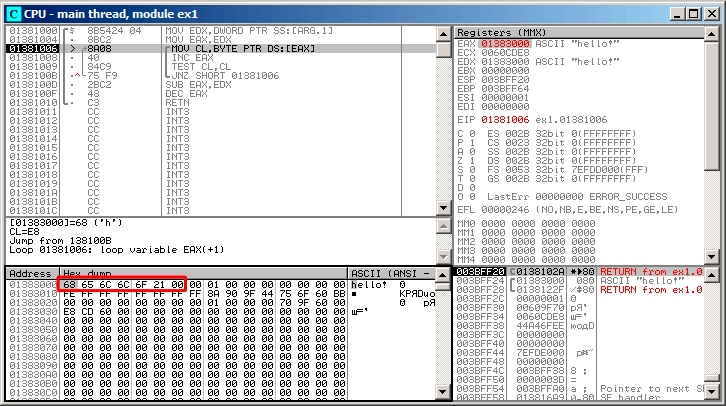
\includegraphics[scale=\FigScale]{patterns/10_strings/1_strlen/olly1.png}
\caption{\olly: \RU{начало первой итерации}\EN{first iteration begin}}
\label{fig:strlen_olly_1}
\end{figure}

\RU{Видно, что \olly обнаружил цикл и, для удобства, \IT{свернула} инструкции тела цикла в скобке}
\EN{We see that \olly found a loop and, for convenience, \IT{wrapped} its instructions in bracket}.
\RU{Нажав правой кнопкой на}\EN{By clicking right button on} \EAX, \RU{можно выбрать}\EN{we can choose} 
``Follow in Dump'' \RU{и позиция в окне памяти будет как раз там, где надо}
\EN{and the memory window position will scroll to the right place}.
\RU{Здесь мы видим в памяти строку}\EN{We can see here a string} ``hello!''\EN{ in memory}.
\RU{После нее имеется как минимум 1 нулевой байт, затем случайный мусор}\EN{There are at least
one zero byte after it and then random garbage}.
\RU{Если \olly видит что в регистре содержится адрес какой-то строки, он показывает эту строку.}
\EN{If \olly sees a register with a valid address in it, pointing to some string, it will show a string.}

\clearpage
\RU{Нажмем}\EN{Let's press} F8 (\stepover) \RU{столько раз, чтобы текущий адрес снова был 
в начале тела цикла}\EN{enough number of times, so the current address will be at the loop body begin again}:

\begin{figure}[H]
\centering
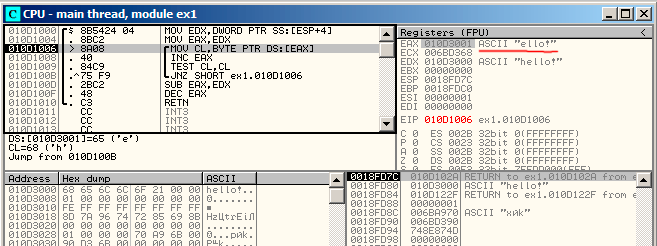
\includegraphics[scale=\FigScale]{patterns/10_strings/1_strlen/olly2.png}
\caption{\olly: \RU{начало второй итерации}\EN{second iteration begin}}
\label{fig:strlen_olly_2}
\end{figure}

\RU{Видно, что}\EN{We see that} \EAX \RU{уже содержит адрес второго символа в строке}
\EN{contain address of the second character in the string}.

\clearpage
\RU{Будем нажимать F8 достаточное количество раз, чтобы выйти из цикла:}
\EN{We will press F8 enough number of times in order to escape from the loop:}

\begin{figure}[H]
\centering
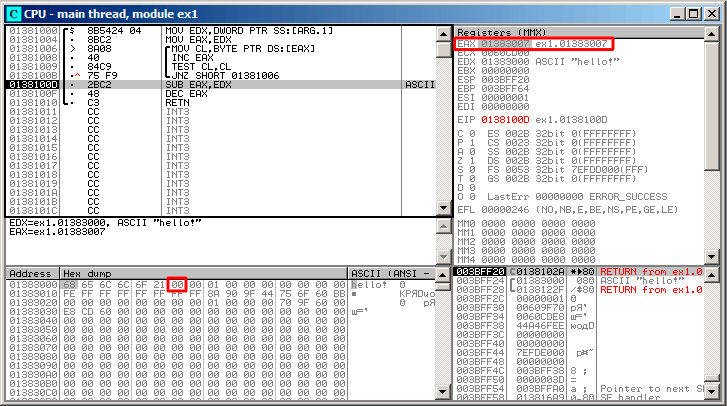
\includegraphics[scale=\FigScale]{patterns/10_strings/1_strlen/olly3.png}
\caption{\olly: \RU{сейчас будет вычисление разницы указателей}\EN{pointers difference to be calculated now}}
\label{fig:strlen_olly_3}
\end{figure}

\RU{Увидим, что \EAX теперь содержит адрес нулевого байта, следующего сразу за строкой}
\EN{We will see that \EAX now contain address of zeroth byte, placed right after the string}.
\RU{А \EDX так и не менялся, он всё еще указывает на начало строки}\EN{Meanwhile, \EDX wasn't changed,
so it still pointing to the string begin}.
\RU{Здесь сейчас будет вычисляться разница между этими двумя адресами}
\EN{Difference between these two addresses will be calculated now}.

\clearpage
\RU{Инструкция \SUB исполнилась}\EN{\SUB instruction was just executed}:

\begin{figure}[H]
\centering
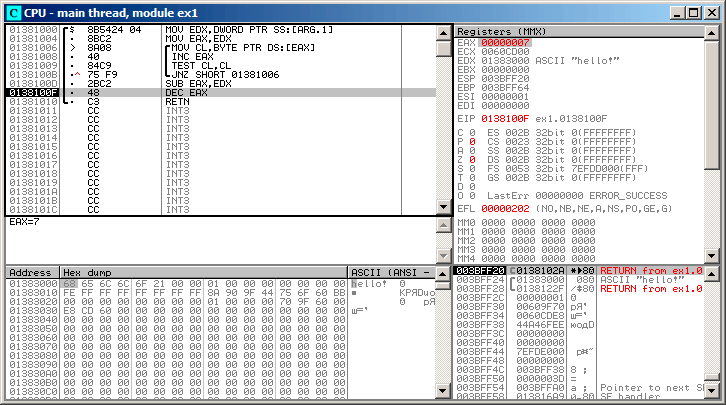
\includegraphics[scale=\FigScale]{patterns/10_strings/1_strlen/olly4.png}
\caption{\olly: \RU{сейчас будет декремент \EAX}\EN{\EAX to be decremented now}}
\label{fig:strlen_olly_4}
\end{figure}

\RU{Разница указателей сейчас в регистре \EAX --- 7.}
\EN{Difference of pointers in the \EAX register now---7.}
\RU{Действительно, длина строки}\EN{Indeed, the} ``hello!'' \RU{--- 6}\EN{string length is 6}, 
\RU{но вместе с нулевым байтом}\EN{but with zeroth byte included}\EMDASH{}7.
\RU{Но}\EN{But the} \TT{strlen()} 
\RU{должна возвращать количество ненулевых символов в строке.}
\EN{must return number of non-zero characters in the string.}
\RU{Так что сейчас будет исполняться декремент и выход из ф-ции}\EN{So the decrement will processed
now and then return from the function}.
